%**************************************************************************
%* SpringSim 2017 Author Kit
%*
%* Word Processing System: TeXnicCenter and MiKTeX
%*
%**************************************************************************

\documentclass{scspaperproc}

\usepackage{latexsym}
\usepackage{graphicx}
\usepackage{mathptmx}
\usepackage{amsmath}
\usepackage{amsfonts}
\usepackage{amssymb}
\usepackage{amsbsy}
\usepackage{amsthm}
%\usepackage[pdftex,colorlinks=true,urlcolor=blue,citecolor=black,anchorcolor=black,linkcolor=black]{hyperref}
%% \usepackage[dvips,colorlinks=true,urlcolor=blue,citecolor=black,%
%% anchorcolor=black,linkcolor=black]{hyperref}

% custom hyphenation rules
\usepackage{hyphenat}
\hyphenation{op-tical net-works semi-conduc-tor}

% theorem style
\newtheoremstyle{scsthe}% hnamei
{8pt}% hSpace abovei
{8pt}% hSpace belowi
{\it}% hBody fonti
{}% hIndent amounti1
{\bf}% hTheorem head fontbf
{.}% hPunctuation after theorem headi
{.5em}% hSpace after theorem headi2
{}% hTheorem head spec (can be left empty, meaning `normal')i
\theoremstyle{scsthe}
\newtheorem{theorem}{Theorem}
\renewcommand{\thetheorem}{\arabic{theorem}}
\newtheorem{corollary}[theorem]{Corollary}
\renewcommand{\thecorollary}{\arabic{corollary}}
\newtheorem{definition}{Definition}
\renewcommand{\thedefinition}{\arabic{definition}}

% avoid overrunning the right margin
\sloppy

%% ***** NOTE *****

%% The use of the long citation format (e.g. "Brown and Edwards
%% (1993)" rather than "[5]") and at the same time using the hyperref
%% package can lead to hard to trace bugs in case the citation is
%% broken accross the line (usually this will mark the entire
%% paragraph as a hyperlink (clickable) which is easily noticeable and
%% fixed if using colorlinks, but not if the color is black -- as it
%% is now). Worse yet, if a citation spans page boundary, LaTeX
%% compilation can fail, with an obscure error message. Since this
%% depends a lot on the flow of the text and wording, these bugs come
%% and go and can be extremely hard for a beginner to trace. The error
%% message can look like this:
%%
%%    ! pdfTeX error (ext4): \pdfendlink ended up in different nesting
%%    level than \pdfstartlink.  \AtBegShi@Output ...ipout \box
%%    \AtBeginShipoutBox \fi \fi
%%    l.174 
%%    ! ==> Fatal error occurred, no output PDF file produced!
%%
%% and can be universally fixed by putting an \mbox{} around the
%% citation in question (in this case, at line 174) and maybe adapting
%% the wording a little bit to improve the paragraph typesetting,
%% which is perhaps not immediately obvious.
%****************************************************************************

% begin document
\begin{document}

% Page header (author list)
\SCSpagesetup{Lux, Watson, Chang, Bernard, Li, Xu, Back, Butt, Cameron, and Hong}

% Conference info
\def\SCSconferenceacro{SpringSim}
\def\SCSpublicationyear{2018}
\def\SCSconferencedates{April 15-18}
\def\SCSconferencevenue{Baltimore, MD, USA}
\def\SCSsymposiumacro{HPC} % High Performance Computing Symposium

% title
\title{Predictive Modeling of I/O Characteristics \\ in High
  Performance Computing Systems}

% AUTHOR LIST
% *** NOTE: May need to adjust titlevboxsize in the preamble
\author{Thomas C. H. Lux \\ [12pt]
Dept. of Computer Science \\
Virginia Polytechnic Institute\\
\& State University \\
Blacksburg, VA 24061 \\
tchlux@vt.edu \\
\and
Layne T. Watson \\[12pt]
Dept. of Computer Science\\
Dept. of Mathematics\\
Dept. of Aerospace \& Ocean Eng.\\ 
Virginia Polytechnic Institute\\
\& State University \\
\and
Tyler H. Chang\\
Jon Bernard\\
Bo Li\\[12pt]
Dept. of Computer Science\\ 
Virginia Polytechnic Institute\\
\& State University \\
\and
Li Xu\\[12pt]
Dept. of Statistics\\ 
Virginia Polytechnic Institute\\
\& State University \\
\and
Godmar Back\\
Ali R. Butt\\
Kirk W. Cameron\\[12pt]
Dept. of Computer Science\\ 
Virginia Polytechnic Institute\\
\& State University \\
\and
Yili Hong\\[12pt]
Dept. of Statistics\\ 
Virginia Polytechnic Institute\\
\& State University \\
}

\maketitle

\section*{Abstract}

Each of high performance computing, cloud computing, and computer
security have their own interests in modeling and predicting the
performance of computers with respect to how they are configured. An
effective model might infer internal mechanics, minimize power
consumption, or maximize computational throughput of a given
system. This paper analyzes a seven-dimensional dataset measuring the
input/output (I/O) characteristics of a cluster of identical computers
using the benchmark IOzone. The I/O performance characteristics are
modeled with respect to system configuration using multivariate
interpolation and approximation techniques. The analysis reveals that
accurate models of I/O characteristics for a computer system may be
created from a small fraction of possible configurations, and that
some modeling techniques will continue to perform well as the number
of system parameters being modeled increases. These results have
strong implications for future predictive analyses based on more
comprehensive sets of system parameters.

\textbf{Keywords:} Regression, approximation, interpolation,
performance modeling


%     Introduction     
%======================
\section{Introduction}

Performance tuning is often an experimentally complex and time-intense
chore necessary for configuring HPC systems. The procedures for this
tuning vary largely from system to system and are often subjectively
guided by the system engineer(s). Once a desired level of performance
is achieved, HPC systems often remain in that base configuration with
all subsequent modifications being incremental. Future changes made
are often associated with updates and job-specific customizations. In
the case that a system has changing workloads or non-stationary
performance objectives that range from maximizing computational
throughput to minimizing power consumption and system variability, it
becomes obvious that a more effective and automated tool is needed for
configuring systems. This scenario presents a challenging and
important application of multivariate approximation and interpolation
techniques.


\begin{enumerate}
\item The value of multivariate Modeling
\item The data context
\item The proposed method for using multivariate models
\item The impact of effective models
\end{enumerate}

This paper compares five multivariate approximation techniques that
operate on inputs in $\mathbb{R}^d$ (vectors of $d$ real numbers) and
produce predicted responses in $\mathbb{R}^1$. In order to provide
coverage of the varied mathematical strategies that can be employed to
solve the continuous modeling problem, three of the techniques are
regression-based and the remaining two techniques produce
interpolants. The sections below outline the mathematical formulations
of each technique and provide computational complexity bounds.

\subsection{Approximation}
\subsubsection{Multivariate Adaptive Regression Splines}
\subsubsection{Multi-Layer Perceptron Regressor}
\subsubsection{Support Vector Regressor}

\subsection{Interpolation}
\subsubsection{Delaunay}
\subsubsection{Linear Shepard}

The remainder of the paper is broken up into \_ parts. \textit{(will
  fill in the parts and descriptions once they are finalized)}

%     Related Work     
%======================
\section{Related Work}
\begin{enumerate}
\item Not sure how much to include here? Shooting for thoroughness or
  simply necessary coverage? How much background should I expect the
  readers of this paper to have in the ``multivariate modeling of
  systems'' area?
\end{enumerate}


%     Methodology     
%=====================
\section{Methodology}
\subsection{Data}

\begin{table}
  \centering
  \begin{tabular}{|c|c|}
    
  \end{tabular}
  \caption{}
  \label{tab:data_type}
\end{table}

\subsection{Dimensional Analysis}
This work utilizes an extension to standard k-fold cross validation
that allows for a more thorough investigation of the expected model
performance in a variety of real-world situations. Alongside
randomized splits, two extra components are considered: the amount of
training data provided, and the dimension of the input data. It is
important to consider that algorithms which perform well with less
training input also require less experimentation. Although, the amount
of training data required may change as a function of the number of
input dimensions and this needs to be studied as well.

\begin{enumerate}
\item Cycling the categorical settings
\item Selecting subsets of 1,2,3 up to 4 dimensions
\item Cycling different training : testing ratios (5:95 $\rightarrow$ 95:5)
\item Generating 200 random training : testing splits
\item Ensuring the testing points are on/inside the convex hull of the training.
\item Ensuring the training points are well-spaced.
\end{enumerate}

\subsection{Prediction}
\begin{enumerate}
\item For each file generated from the dimensional analysis, train on
  the training data, evaluate at the testing data points
\end{enumerate}


%     Results     
%=================
\section{Results}
\subsection{I/O Throughput Mean}

%% \begin{center}
%%   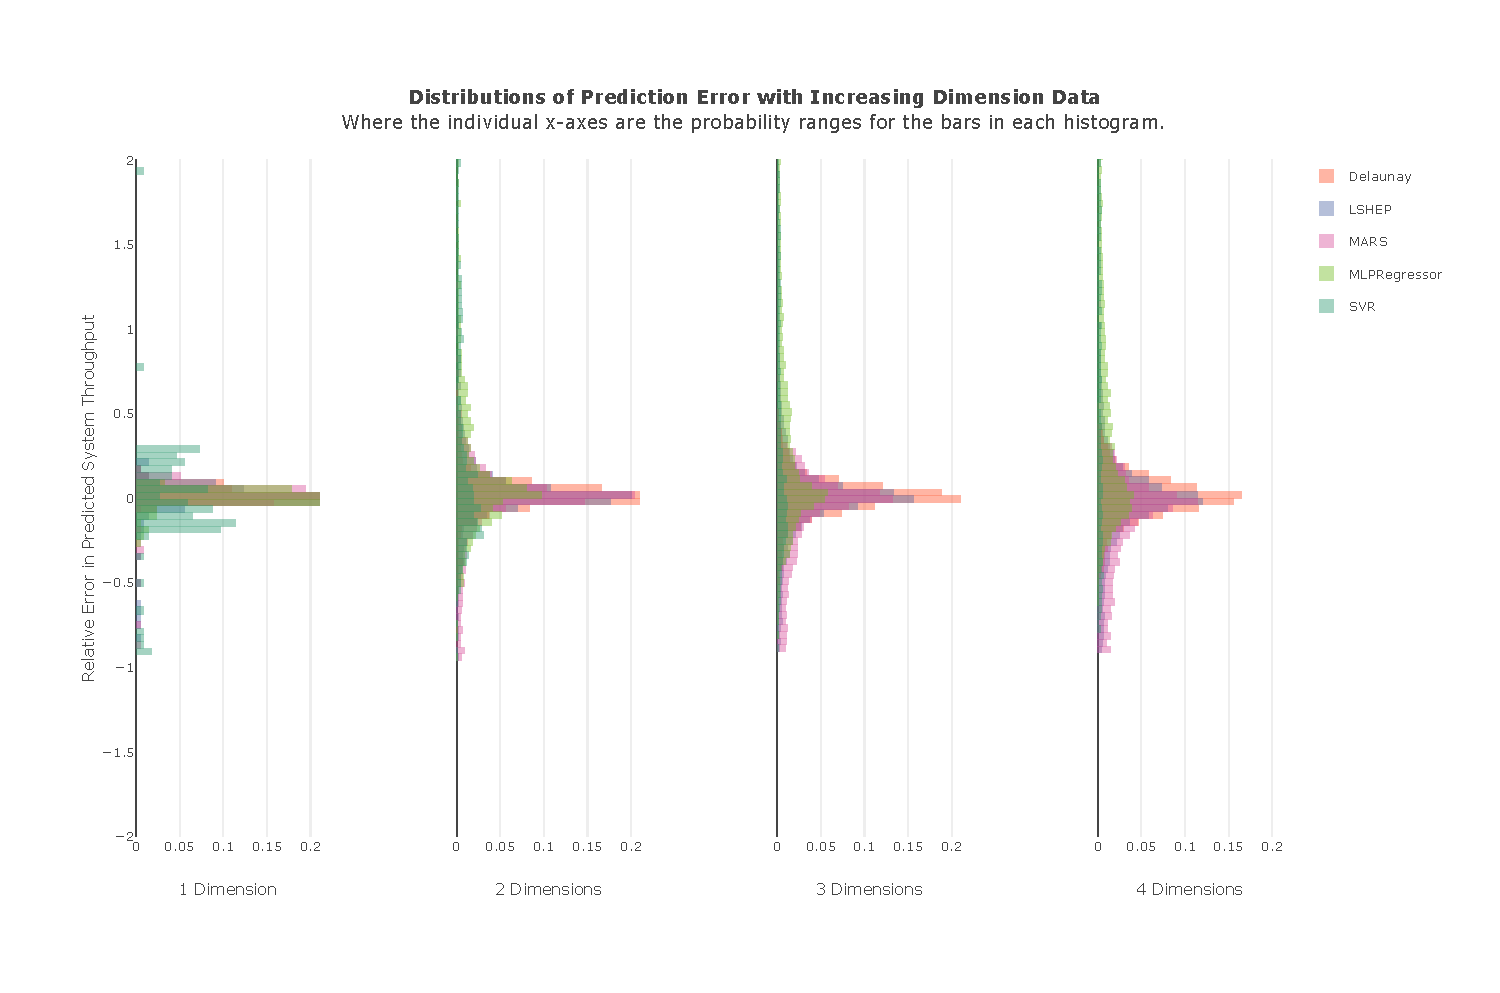
\includegraphics[width=\textwidth]{Prediction_Performance_Dim.pdf}
%%   \caption{In this figure we see how the distribution of errors }
%% \end{center}

\begin{figure}
  \centering
  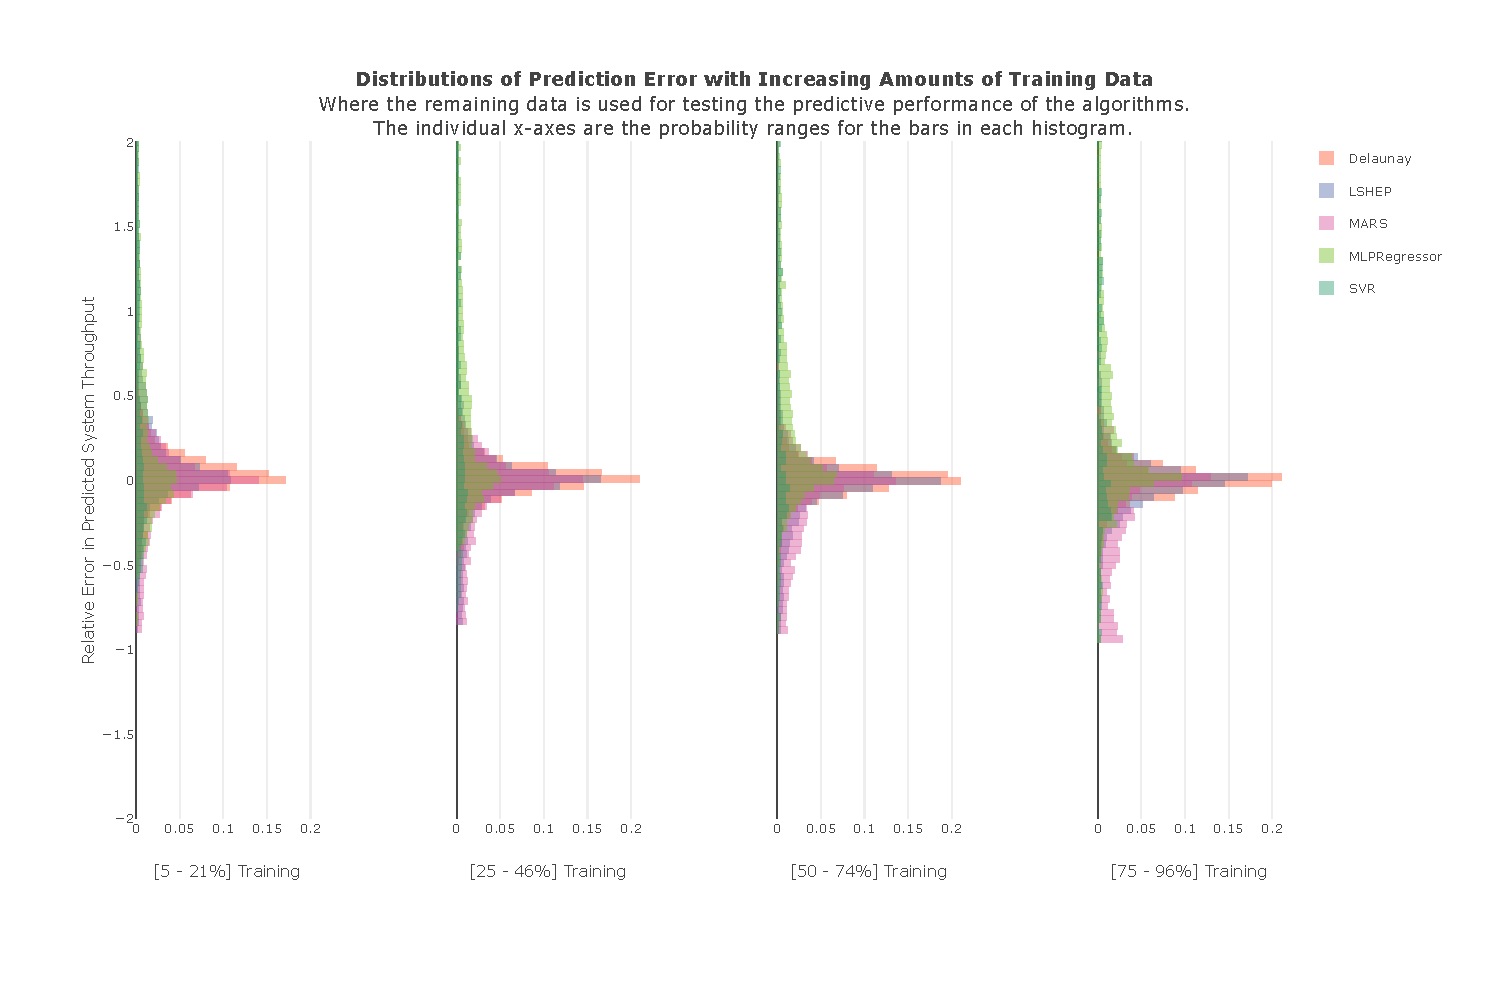
\includegraphics[width=\textwidth]{Prediction_Performance_TT_Ratio.pdf}
  \caption{In this figure, it can be seen how the distribution of
    prediction errors for each algorithm is affected by the quantity
    of training data provided. Notice that for all amounts of training
    data, Delaunay has the largest likelihoods around 0 error.}
  \label{fig:tt_ratio}
\end{figure}

\begin{table}
  \centering
  \begin{tabular}{|c||c|c|c|}
    %% \hline
    %% \multicolumn{4}{|c|}{Table Title}\\
    \hline
    \textbf{Algorithm} & \textbf{Input Dimension} & \textbf{Mean Absolute Error} & \textbf{Mean Relative Error}\\
    \hline
    Delaunay     & 1 & 2060267   & 0.03 \\
                 & 2 & 2916224   & 0.07 \\
                 & 3 & 3001794   & 0.09 \\
                 & 4 & 3134779   & 0.10 \\
    \hline
    LSHEP        & 1 & 6353148   & 0.06 \\
                 & 2 & 13038882  & 1.52 \\
                 & 3 & 5446207   & 1.13 \\
                 & 4 & 5133648   & 1.07 \\
    \hline
    MARS         & 1 & 2176368   & 0.03 \\
                 & 2 & 6213369   & 0.61 \\
                 & 3 & 4024964   & 0.65 \\
                 & 4 & 4497414   & 1.01 \\
    \hline
    MLPRegressor & 1 & 2461097   & 0.06 \\
                 & 2 & 8883580   & 0.81 \\
                 & 3 & 11190977  & 2.03 \\
                 & 4 & 11831721  & 2.20 \\
    \hline
    SVR          & 1 & 19306731  & 0.96 \\
                 & 2 & 78213963  & 18.49\\
                 & 3 & 97761266  & 31.27\\
                 & 4 & 113551300 & 37.2 \\
    \hline
  \end{tabular}
  \caption{Most models experience a decay in predictive performance as
    the dimension of the data increases. This is expected because
    higher dimension input has exponentially more possible patterns to
    identify. The MLP Regressor and SVR experience the worst decay in
    performance with increasing dimension.}
  \label{tab:perf_by_dim}
\end{table}

\begin{table}
  \centering
  \begin{tabular}{|c||c|c|c|}
    %% \hline
    %% \multicolumn{4}{|c|}{Table Title}\\
    \hline
    \textbf{Algorithm} & \textbf{Training Data} & \textbf{Mean Absolute Error} & \textbf{Mean Relative Error}\\
    \hline
    Delaunay     & [5-21]\%  & 5274933   & 0.11 \\
                 & [25-46]\% & 2898330   & 0.08 \\
                 & [50-74]\% & 1518477   & 0.07 \\
                 & [75-96]\% & 886346    & 0.08 \\
    \hline
    LSHEP        & [5-21]\%  & 13218469  & 2.53 \\
                 & [25-46]\% & 4936381   & 0.85 \\
                 & [50-74]\% & 2251409   & 0.26 \\
                 & [75-96]\% & 1415034   & 0.15 \\
    \hline
    MARS         & [5-21]\%  & 6543153   & 0.61 \\
                 & [25-46]\% & 4324916   & 0.80 \\
                 & [50-74]\% & 3115943   & 0.95 \\
                 & [75-96]\% & 2591451   & 0.74 \\
    \hline
    MLPRegressor & [5-21]\%  & 17348982  & 2.58 \\
                 & [25-46]\% & 12504957  & 2.29 \\
                 & [50-74]\% & 5292177   & 1.17 \\
                 & [75-96]\% & 2996253   & 1.02 \\
    \hline
    SVR          & [5-21]\%  & 170906944 & 49.45\\
                 & [25-46]\% & 99851846  & 31.28\\
                 & [50-74]\% & 51565405  & 19.63\\
                 & [75-96]\% & 27125130  & 12.6 \\
    \hline
  \end{tabular}
  \caption{All models experience a reduction in error with increasing
    amounts of training data. This suggests that the data being
    modeled is pattern-dense, over-fitting is \textit{not} occurring,
    and that oversimplifications will tend towards worse predictions.}
  \label{tab:perf_by_tt}
\end{table}

\subsection{I/O Throughput Variance}
\subsection{Increasing Dimension}


%     Discussion     
%====================
\section{Discussion}
\subsection{Modeling the System}
\subsection{Quantifying Variability}
\subsection{Extending the Analysis}

%     Future Work     
%=====================
\section{Future Work}


\bibliographystyle{scsproc}
\bibliography{paper}

\end{document}


%%  ALGORITHM     MEAN ABSOLUTE ERROR    MEAN RELATIVE ERROR
                                                      
%% 1 Dimension                                        
%%  Delaunay         2060267             0.03 
%%  MARS             2176368             0.03 
%%  MLPRegressor     2461097             0.06 
%%  LSHEP            6353148             0.06 
%%  SVR             19306731             0.96 
                                                      
%% 2 Dimensions                                       
%%  Delaunay         2916224             0.07 
%%  MARS             6213369             0.61 
%%  MLPRegressor     8883580             0.81 
%%  LSHEP           13038882             1.52 
%%  SVR             78213963             18.49
                                                      
%% 3 Dimensions                                       
%%  Delaunay         3001794             0.09 
%%  MARS             4024964             0.65 
%%  LSHEP            5446207             1.13 
%%  MLPRegressor    11190977             2.03 
%%  SVR             97761266             31.27
                                                      
%% 4 Dimensions                                       
%%  Delaunay         3134779             0.10 
%%  MARS             4497414             1.01 
%%  LSHEP            5133648             1.07 
%%  MLPRegressor    11831721             2.20 
%%  SVR            113551300             37.26
                                                      
%% [5 - 21%] Training Data               
%%  Delaunay         5274933             0.11 
%%  MARS             6543153             0.61 
%%  LSHEP           13218469             2.53 
%%  MLPRegressor    17348982             2.58 
%%  SVR            170906944             49.45
                                                      
%% [25 - 46%] Training Data              
%%  Delaunay         2898330             0.08 
%%  MARS             4324916             0.80 
%%  LSHEP            4936381             0.85 
%%  MLPRegressor    12504957             2.29 
%%  SVR             99851846             31.28
                                                      
%% [50 - 74%] Training Data              
%%  Delaunay         1518477             0.07 
%%  LSHEP            2251409             0.26 
%%  MARS             3115943             0.95 
%%  MLPRegressor     5292177             1.17 
%%  SVR             51565405             19.63
                                                      
%% [75 - 96%] Training Data              
%%  Delaunay          886346             0.08 
%%  LSHEP            1415034             0.15 
%%  MARS             2591451             0.74 
%%  MLPRegressor     2996253             1.02 
%%  SVR             27125130             12.64
                                                      
                                                      
%% ALGORITHM   AVG ABSOLUTE MEAN ERROR   AVG RELATIVE ERROR
%% Delaunay         2711394              0.08  
%% MARS             4185947              0.72  
%% LSHEP            6474147              0.94  
%% MLPRegressor     9063718              1.48  
%% SVR             82285323              25.12 

